% Created by tikzDevice version 0.9 on 2016-02-03 14:10:02
% !TEX encoding = UTF-8 Unicode
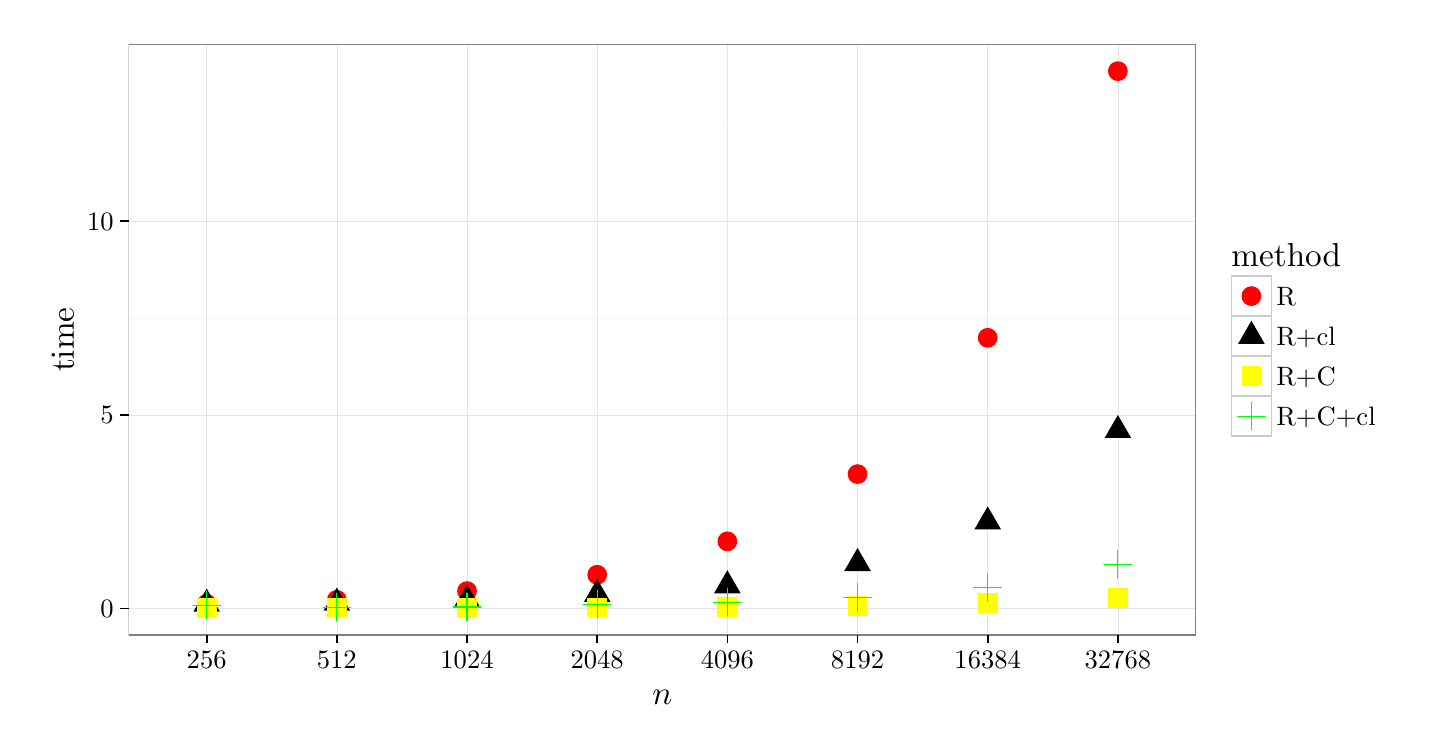
\begin{tikzpicture}[x=1pt,y=1pt]
\definecolor{fillColor}{RGB}{255,255,255}
\path[use as bounding box,fill=fillColor,fill opacity=0.00] (0,0) rectangle (505.89,252.94);
\begin{scope}
\path[clip] (  0.00,  0.00) rectangle (505.89,252.94);
\definecolor{drawColor}{RGB}{255,255,255}
\definecolor{fillColor}{RGB}{255,255,255}

\path[draw=drawColor,line width= 0.6pt,line join=round,line cap=round,fill=fillColor] (  0.00,  0.00) rectangle (505.89,252.95);
\end{scope}
\begin{scope}
\path[clip] ( 36.46, 33.48) rectangle (422.16,246.94);
\definecolor{fillColor}{RGB}{255,255,255}

\path[fill=fillColor] ( 36.46, 33.48) rectangle (422.16,246.94);
\definecolor{drawColor}{gray}{0.98}

\path[draw=drawColor,line width= 0.6pt,line join=round] ( 36.46, 78.08) --
	(422.16, 78.08);

\path[draw=drawColor,line width= 0.6pt,line join=round] ( 36.46,148.02) --
	(422.16,148.02);

\path[draw=drawColor,line width= 0.6pt,line join=round] ( 36.46,217.96) --
	(422.16,217.96);
\definecolor{drawColor}{gray}{0.90}

\path[draw=drawColor,line width= 0.2pt,line join=round] ( 36.46, 43.11) --
	(422.16, 43.11);

\path[draw=drawColor,line width= 0.2pt,line join=round] ( 36.46,113.05) --
	(422.16,113.05);

\path[draw=drawColor,line width= 0.2pt,line join=round] ( 36.46,182.99) --
	(422.16,182.99);

\path[draw=drawColor,line width= 0.2pt,line join=round] ( 64.68, 33.48) --
	( 64.68,246.94);

\path[draw=drawColor,line width= 0.2pt,line join=round] (111.72, 33.48) --
	(111.72,246.94);

\path[draw=drawColor,line width= 0.2pt,line join=round] (158.76, 33.48) --
	(158.76,246.94);

\path[draw=drawColor,line width= 0.2pt,line join=round] (205.79, 33.48) --
	(205.79,246.94);

\path[draw=drawColor,line width= 0.2pt,line join=round] (252.83, 33.48) --
	(252.83,246.94);

\path[draw=drawColor,line width= 0.2pt,line join=round] (299.87, 33.48) --
	(299.87,246.94);

\path[draw=drawColor,line width= 0.2pt,line join=round] (346.90, 33.48) --
	(346.90,246.94);

\path[draw=drawColor,line width= 0.2pt,line join=round] (393.94, 33.48) --
	(393.94,246.94);
\definecolor{fillColor}{RGB}{255,0,0}

\path[fill=fillColor] ( 64.68, 44.74) circle (  3.57);

\path[fill=fillColor] (111.72, 46.19) circle (  3.57);

\path[fill=fillColor] (158.76, 49.36) circle (  3.57);

\path[fill=fillColor] (205.79, 55.25) circle (  3.57);

\path[fill=fillColor] (252.83, 67.32) circle (  3.57);

\path[fill=fillColor] (299.87, 91.62) circle (  3.57);

\path[fill=fillColor] (346.90,140.87) circle (  3.57);

\path[fill=fillColor] (393.94,237.24) circle (  3.57);
\definecolor{fillColor}{RGB}{0,0,0}

\path[fill=fillColor] ( 64.68, 50.23) --
	( 69.49, 41.90) --
	( 59.88, 41.90) --
	cycle;

\path[fill=fillColor] (111.72, 50.63) --
	(116.53, 42.30) --
	(106.92, 42.30) --
	cycle;

\path[fill=fillColor] (158.76, 51.73) --
	(163.56, 43.41) --
	(153.95, 43.41) --
	cycle;

\path[fill=fillColor] (205.79, 53.76) --
	(210.60, 45.44) --
	(200.99, 45.44) --
	cycle;

\path[fill=fillColor] (252.83, 56.88) --
	(257.64, 48.56) --
	(248.03, 48.56) --
	cycle;

\path[fill=fillColor] (299.87, 64.93) --
	(304.67, 56.60) --
	(295.06, 56.60) --
	cycle;

\path[fill=fillColor] (346.90, 79.98) --
	(351.71, 71.65) --
	(342.10, 71.65) --
	cycle;

\path[fill=fillColor] (393.94,112.99) --
	(398.75,104.67) --
	(389.14,104.67) --
	cycle;
\definecolor{fillColor}{RGB}{255,255,0}

\path[fill=fillColor] ( 61.12, 39.61) --
	( 68.25, 39.61) --
	( 68.25, 46.75) --
	( 61.12, 46.75) --
	cycle;

\path[fill=fillColor] (108.15, 39.64) --
	(115.29, 39.64) --
	(115.29, 46.78) --
	(108.15, 46.78) --
	cycle;

\path[fill=fillColor] (155.19, 39.69) --
	(162.33, 39.69) --
	(162.33, 46.83) --
	(155.19, 46.83) --
	cycle;

\path[fill=fillColor] (202.23, 39.81) --
	(209.36, 39.81) --
	(209.36, 46.95) --
	(202.23, 46.95) --
	cycle;

\path[fill=fillColor] (249.26, 40.03) --
	(256.40, 40.03) --
	(256.40, 47.17) --
	(249.26, 47.17) --
	cycle;

\path[fill=fillColor] (296.30, 40.52) --
	(303.44, 40.52) --
	(303.44, 47.65) --
	(296.30, 47.65) --
	cycle;

\path[fill=fillColor] (343.34, 41.40) --
	(350.47, 41.40) --
	(350.47, 48.54) --
	(343.34, 48.54) --
	cycle;

\path[fill=fillColor] (390.37, 43.35) --
	(397.51, 43.35) --
	(397.51, 50.49) --
	(390.37, 50.49) --
	cycle;
\definecolor{drawColor}{RGB}{0,255,0}

\path[draw=drawColor,line width= 0.4pt,line join=round,line cap=round] ( 59.64, 44.29) -- ( 69.73, 44.29);

\path[draw=drawColor,line width= 0.4pt,line join=round,line cap=round] ( 64.68, 39.24) -- ( 64.68, 49.34);

\path[draw=drawColor,line width= 0.4pt,line join=round,line cap=round] (106.67, 43.54) -- (116.77, 43.54);

\path[draw=drawColor,line width= 0.4pt,line join=round,line cap=round] (111.72, 38.49) -- (111.72, 48.58);

\path[draw=drawColor,line width= 0.4pt,line join=round,line cap=round] (153.71, 43.61) -- (163.80, 43.61);

\path[draw=drawColor,line width= 0.4pt,line join=round,line cap=round] (158.76, 38.56) -- (158.76, 48.65);

\path[draw=drawColor,line width= 0.4pt,line join=round,line cap=round] (200.75, 44.60) -- (210.84, 44.60);

\path[draw=drawColor,line width= 0.4pt,line join=round,line cap=round] (205.79, 39.56) -- (205.79, 49.65);

\path[draw=drawColor,line width= 0.4pt,line join=round,line cap=round] (247.78, 45.33) -- (257.88, 45.33);

\path[draw=drawColor,line width= 0.4pt,line join=round,line cap=round] (252.83, 40.28) -- (252.83, 50.37);

\path[draw=drawColor,line width= 0.4pt,line join=round,line cap=round] (294.82, 47.04) -- (304.91, 47.04);

\path[draw=drawColor,line width= 0.4pt,line join=round,line cap=round] (299.87, 41.99) -- (299.87, 52.09);

\path[draw=drawColor,line width= 0.4pt,line join=round,line cap=round] (341.86, 50.69) -- (351.95, 50.69);

\path[draw=drawColor,line width= 0.4pt,line join=round,line cap=round] (346.90, 45.65) -- (346.90, 55.74);

\path[draw=drawColor,line width= 0.4pt,line join=round,line cap=round] (388.89, 58.97) -- (398.99, 58.97);

\path[draw=drawColor,line width= 0.4pt,line join=round,line cap=round] (393.94, 53.92) -- (393.94, 64.02);
\definecolor{drawColor}{gray}{0.50}

\path[draw=drawColor,line width= 0.6pt,line join=round,line cap=round] ( 36.46, 33.48) rectangle (422.16,246.94);
\end{scope}
\begin{scope}
\path[clip] (  0.00,  0.00) rectangle (505.89,252.94);
\definecolor{drawColor}{RGB}{0,0,0}

\node[text=drawColor,anchor=base east,inner sep=0pt, outer sep=0pt, scale=  0.96] at ( 31.06, 39.80) {0};

\node[text=drawColor,anchor=base east,inner sep=0pt, outer sep=0pt, scale=  0.96] at ( 31.06,109.74) {5};

\node[text=drawColor,anchor=base east,inner sep=0pt, outer sep=0pt, scale=  0.96] at ( 31.06,179.69) {10};
\end{scope}
\begin{scope}
\path[clip] (  0.00,  0.00) rectangle (505.89,252.94);
\definecolor{drawColor}{RGB}{0,0,0}

\path[draw=drawColor,line width= 0.6pt,line join=round] ( 33.46, 43.11) --
	( 36.46, 43.11);

\path[draw=drawColor,line width= 0.6pt,line join=round] ( 33.46,113.05) --
	( 36.46,113.05);

\path[draw=drawColor,line width= 0.6pt,line join=round] ( 33.46,182.99) --
	( 36.46,182.99);
\end{scope}
\begin{scope}
\path[clip] (  0.00,  0.00) rectangle (505.89,252.94);
\definecolor{drawColor}{RGB}{0,0,0}

\path[draw=drawColor,line width= 0.6pt,line join=round] ( 64.68, 30.48) --
	( 64.68, 33.48);

\path[draw=drawColor,line width= 0.6pt,line join=round] (111.72, 30.48) --
	(111.72, 33.48);

\path[draw=drawColor,line width= 0.6pt,line join=round] (158.76, 30.48) --
	(158.76, 33.48);

\path[draw=drawColor,line width= 0.6pt,line join=round] (205.79, 30.48) --
	(205.79, 33.48);

\path[draw=drawColor,line width= 0.6pt,line join=round] (252.83, 30.48) --
	(252.83, 33.48);

\path[draw=drawColor,line width= 0.6pt,line join=round] (299.87, 30.48) --
	(299.87, 33.48);

\path[draw=drawColor,line width= 0.6pt,line join=round] (346.90, 30.48) --
	(346.90, 33.48);

\path[draw=drawColor,line width= 0.6pt,line join=round] (393.94, 30.48) --
	(393.94, 33.48);
\end{scope}
\begin{scope}
\path[clip] (  0.00,  0.00) rectangle (505.89,252.94);
\definecolor{drawColor}{RGB}{0,0,0}

\node[text=drawColor,anchor=base,inner sep=0pt, outer sep=0pt, scale=  0.96] at ( 64.68, 21.46) {256};

\node[text=drawColor,anchor=base,inner sep=0pt, outer sep=0pt, scale=  0.96] at (111.72, 21.46) {512};

\node[text=drawColor,anchor=base,inner sep=0pt, outer sep=0pt, scale=  0.96] at (158.76, 21.46) {1024};

\node[text=drawColor,anchor=base,inner sep=0pt, outer sep=0pt, scale=  0.96] at (205.79, 21.46) {2048};

\node[text=drawColor,anchor=base,inner sep=0pt, outer sep=0pt, scale=  0.96] at (252.83, 21.46) {4096};

\node[text=drawColor,anchor=base,inner sep=0pt, outer sep=0pt, scale=  0.96] at (299.87, 21.46) {8192};

\node[text=drawColor,anchor=base,inner sep=0pt, outer sep=0pt, scale=  0.96] at (346.90, 21.46) {16384};

\node[text=drawColor,anchor=base,inner sep=0pt, outer sep=0pt, scale=  0.96] at (393.94, 21.46) {32768};
\end{scope}
\begin{scope}
\path[clip] (  0.00,  0.00) rectangle (505.89,252.94);
\definecolor{drawColor}{RGB}{0,0,0}

\node[text=drawColor,anchor=base,inner sep=0pt, outer sep=0pt, scale=  1.20] at (229.31,  8.40) {$n$};
\end{scope}
\begin{scope}
\path[clip] (  0.00,  0.00) rectangle (505.89,252.94);
\definecolor{drawColor}{RGB}{0,0,0}

\node[text=drawColor,rotate= 90.00,anchor=base,inner sep=0pt, outer sep=0pt, scale=  1.20] at ( 16.66,140.21) {time};
\end{scope}
\begin{scope}
\path[clip] (  0.00,  0.00) rectangle (505.89,252.94);
\definecolor{fillColor}{RGB}{255,255,255}

\path[fill=fillColor] (430.70,101.10) rectangle (491.35,179.33);
\end{scope}
\begin{scope}
\path[clip] (  0.00,  0.00) rectangle (505.89,252.94);
\definecolor{drawColor}{RGB}{0,0,0}

\node[text=drawColor,anchor=base west,inner sep=0pt, outer sep=0pt, scale=  1.20] at (434.97,166.79) {method};
\end{scope}
\begin{scope}
\path[clip] (  0.00,  0.00) rectangle (505.89,252.94);
\definecolor{drawColor}{gray}{0.80}
\definecolor{fillColor}{RGB}{255,255,255}

\path[draw=drawColor,line width= 0.6pt,line join=round,line cap=round,fill=fillColor] (434.97,148.73) rectangle (449.42,163.18);
\end{scope}
\begin{scope}
\path[clip] (  0.00,  0.00) rectangle (505.89,252.94);
\definecolor{fillColor}{RGB}{255,0,0}

\path[fill=fillColor] (442.19,155.95) circle (  3.57);
\end{scope}
\begin{scope}
\path[clip] (  0.00,  0.00) rectangle (505.89,252.94);
\definecolor{drawColor}{gray}{0.80}
\definecolor{fillColor}{RGB}{255,255,255}

\path[draw=drawColor,line width= 0.6pt,line join=round,line cap=round,fill=fillColor] (434.97,134.27) rectangle (449.42,148.73);
\end{scope}
\begin{scope}
\path[clip] (  0.00,  0.00) rectangle (505.89,252.94);
\definecolor{fillColor}{RGB}{0,0,0}

\path[fill=fillColor] (442.19,147.05) --
	(447.00,138.72) --
	(437.39,138.72) --
	cycle;
\end{scope}
\begin{scope}
\path[clip] (  0.00,  0.00) rectangle (505.89,252.94);
\definecolor{drawColor}{gray}{0.80}
\definecolor{fillColor}{RGB}{255,255,255}

\path[draw=drawColor,line width= 0.6pt,line join=round,line cap=round,fill=fillColor] (434.97,119.82) rectangle (449.42,134.27);
\end{scope}
\begin{scope}
\path[clip] (  0.00,  0.00) rectangle (505.89,252.94);
\definecolor{fillColor}{RGB}{255,255,0}

\path[fill=fillColor] (438.63,123.48) --
	(445.76,123.48) --
	(445.76,130.61) --
	(438.63,130.61) --
	cycle;
\end{scope}
\begin{scope}
\path[clip] (  0.00,  0.00) rectangle (505.89,252.94);
\definecolor{drawColor}{gray}{0.80}
\definecolor{fillColor}{RGB}{255,255,255}

\path[draw=drawColor,line width= 0.6pt,line join=round,line cap=round,fill=fillColor] (434.97,105.36) rectangle (449.42,119.82);
\end{scope}
\begin{scope}
\path[clip] (  0.00,  0.00) rectangle (505.89,252.94);
\definecolor{drawColor}{RGB}{0,255,0}

\path[draw=drawColor,line width= 0.4pt,line join=round,line cap=round] (437.15,112.59) -- (447.24,112.59);

\path[draw=drawColor,line width= 0.4pt,line join=round,line cap=round] (442.19,107.54) -- (442.19,117.64);
\end{scope}
\begin{scope}
\path[clip] (  0.00,  0.00) rectangle (505.89,252.94);
\definecolor{drawColor}{RGB}{0,0,0}

\node[text=drawColor,anchor=base west,inner sep=0pt, outer sep=0pt, scale=  0.96] at (451.23,152.65) {R};
\end{scope}
\begin{scope}
\path[clip] (  0.00,  0.00) rectangle (505.89,252.94);
\definecolor{drawColor}{RGB}{0,0,0}

\node[text=drawColor,anchor=base west,inner sep=0pt, outer sep=0pt, scale=  0.96] at (451.23,138.19) {R+cl};
\end{scope}
\begin{scope}
\path[clip] (  0.00,  0.00) rectangle (505.89,252.94);
\definecolor{drawColor}{RGB}{0,0,0}

\node[text=drawColor,anchor=base west,inner sep=0pt, outer sep=0pt, scale=  0.96] at (451.23,123.74) {R+C};
\end{scope}
\begin{scope}
\path[clip] (  0.00,  0.00) rectangle (505.89,252.94);
\definecolor{drawColor}{RGB}{0,0,0}

\node[text=drawColor,anchor=base west,inner sep=0pt, outer sep=0pt, scale=  0.96] at (451.23,109.28) {R+C+cl};
\end{scope}
\end{tikzpicture}
